\section{EMPIRICAL EXAMPLES OF PROPENSITY SCORE MATICHNG IN ACCOUNTING SETTINGS}
監査法人の規模、内部統制、アナリストのフォロー数が財務報告の質に与える影響を検証する。

\subsection*{Sample Selection and Descriptive Statistics}

\paragraph{サンプルの選択}

\begin{itemize}
 \item 期間は、Sarbanes-Oxley (SOX) 法にかかる観測値が取得可能な2004〜2012年である。
 \item 以下の要件に該当するサンプルを除外する。
   \begin{itemize}
    \item 海外企業、および金融業(2桁SICコードの60--69)に属する観測値
    \item 総資産が500ドル以下の観測値
    \item 2桁SICコードに基づく産業年が10観測値未満のもの(裁量的会計発生高を計算するための要件)
    \item 欠損値のある観測値
   \end{itemize}
 \item 最終サンプルは、監査法人の規模の分析とアナリストのフォローの分析で29,227観測値、内部統制の弱さの分析で20,385観測値である。
 \item 最終サンプルの内訳は、以下のとおりである。
    \begin{itemize}
    \item Big 4に監査されている($\mathit{BIG}4_{it}=1$)のが19,988企業年
    \item 少なくとも1つの内部統制の弱さを監査報告書で指摘されている($\mathit{WEAK}_{it}=1$)のが1,422企業年
    \item 少なくとも1人のアナリストがついている($\mathit{ANALYST}_{it}=1$)21,144企業年
   \end{itemize}
\end{itemize}

\paragraph{データソース}

\begin{itemize}
 \item 監査法人、内部統制の弱さ、財務諸表の再報告にかかるデータ:Audit Analytics
 \item アナリストにかかるデータ:the Institutional Brokers’ Estimate System (I/B/E/S)
 \item 財務データ:Compustat
  \begin{itemize}
   \item Table 2:記述統計量
  \end{itemize}
\end{itemize}

\subsection*{Research Design}

$\mathit{BIG}4_{it}$、$\mathit{WEAK}_{it}$、$\mathit{ANALYST}_{it}$のそれぞれを割り当て変数とし、PSMを行い、ATEを推定する。

\paragraph{予測モデル(第1段階)}

\begin{equation}
\mathit{D}_{it} = \alpha_0 + \alpha_1 \mathit{X}_{it} + \varepsilon_{it}
\end{equation}

\begin{itemize}
 \item $\mathit{D}_{it}$は、$\mathit{BIG}4_{it}$、$\mathit{WEAK}_{it}$、$\mathit{ANALYST}_{it}$で、処置群と対照群に割り当てるダミー変数
 \item PSMのキャリパー距離は、0.03とする。
\end{itemize}

\paragraph{結果モデル(第2段階)}

\begin{equation}
\mathit{QUALITY}_{it} = \beta_0 + \beta_1 \mathit{D}_{it} + \beta_2 \mathit{X}_{it} +\varepsilon_{it}
\end{equation}

\begin{itemize}
 \item $\mathit{QUALITY}_{it}$は、財務報告の質を示し、本分析では、裁量的会計発生高($\mathit{ABSACC}_{it}$)、および財務諸表の再報告($\mathit{RESTATE}_{it}$)のそれぞれで評価している。
 \item $X_{it}$は、企業規模($\mathit{LNASSETS}_{it}$)、パフォーマンス($\mathit{ROA}_{it}$、$\mathit{ATURN}_{it}$)、財政状態($\mathit{CURR}_{it}$、$\mathit{LEV}_{it}$、$\mathit{DISTRESS}_{it}$)、設立年数($\mathit{AGE}_{it}$)、成長性($\mathit{GROWTH}_{it}$)、企業価値($\mathit{BTM}_{it}$)、年度固定効果を用いる。
  \begin{itemize}
   \item Appendix B:変数の定義
  \end{itemize}
 \item 本分析で観察したいATEは、(5)式の$\beta_1$で示される。
\end{itemize}

\subsection*{Diagnosing Function Form Misspecification}
\begin{itemize}
 \item MRにおいて、FFMが懸念されるのかについて判定する。
 \item Ramsey(1969)のRESETテストがFFMを見る手法として用いられることがある(Lawrence et al. 2011を見よ)。
 \item ただし、これは、変数の非線形性が追加的な説明を与えているのかどうかについて検証するものであり、結果変数と非線形な関係にある変数がATEの推定にバイアスを与えてるのかどうかを見るものではない。
\end{itemize}

\paragraph{変数を追加してFFMを判定する方法(Table 3)}

\begin{itemize}
 \item ここで、MRにおけるFFMを判定する手法として、コントロール変数(たとえば、変数を2乗したもの、3乗したもの)を追加する手法を提唱する。
 \item もし、元のモデルと変数を追加したモデルの結果が異なるのなら、FFMに対する懸念がある。
 \item (5)式を推定した結果を見ると、変数を追加したとしても((2)列と(5)列)、基本的な結果は元のモデル((1)列と(4)列)大きくは変わらない。
 \item しかし、監査法人の規模とアナリストのフォローで割り当てた場合、Chow(1960)の検定をすると、元のモデルのATEと変数を追加したモデルのATEの間で有意な差が認められる。
  \begin{itemize}
   \item これは、$X$と結果変数が非線形な関係にあることを示す。
  \end{itemize}
\end{itemize}

\subsection*{First-Stage Prediction Model}

\paragraph{第1段階((4)式)の推定結果(Table 4)}

\begin{itemize}
 \item 先行研究では、pseudo-${\rm R^2}$が高ければ高いほど、PSMは良い状態であることが示唆されている。
 \item しかし、この説明力は、割り当てが大きく影響を与えている。
 \item つまり、処置群の$X$が対照群の$X$とより大きく相違しているのなら、回帰式の説明力は大きくなる。
 \item overlapが大きければ大きいほど、pseudo-${\rm R^2}$は小さくなるとも言える。
  \begin{itemize}
   \item ただし、説明力がPSMの有効性を必ずしも示しているわけではない。
  \end{itemize}
\end{itemize}

\subsection*{Demonstration of Propensity Score Overlap}

処置群と対照群の傾向スコアのoverlapについて確認するため、Shaikh, Simonsen, Vydacil, and Yildiz(2009)と同様に、傾向スコアの密度をプロットする。

\paragraph{監査法人の規模で割り当てた場合の傾向スコアのプロット(Figure 1, Panel A)}

\begin{figure}
 \centering
 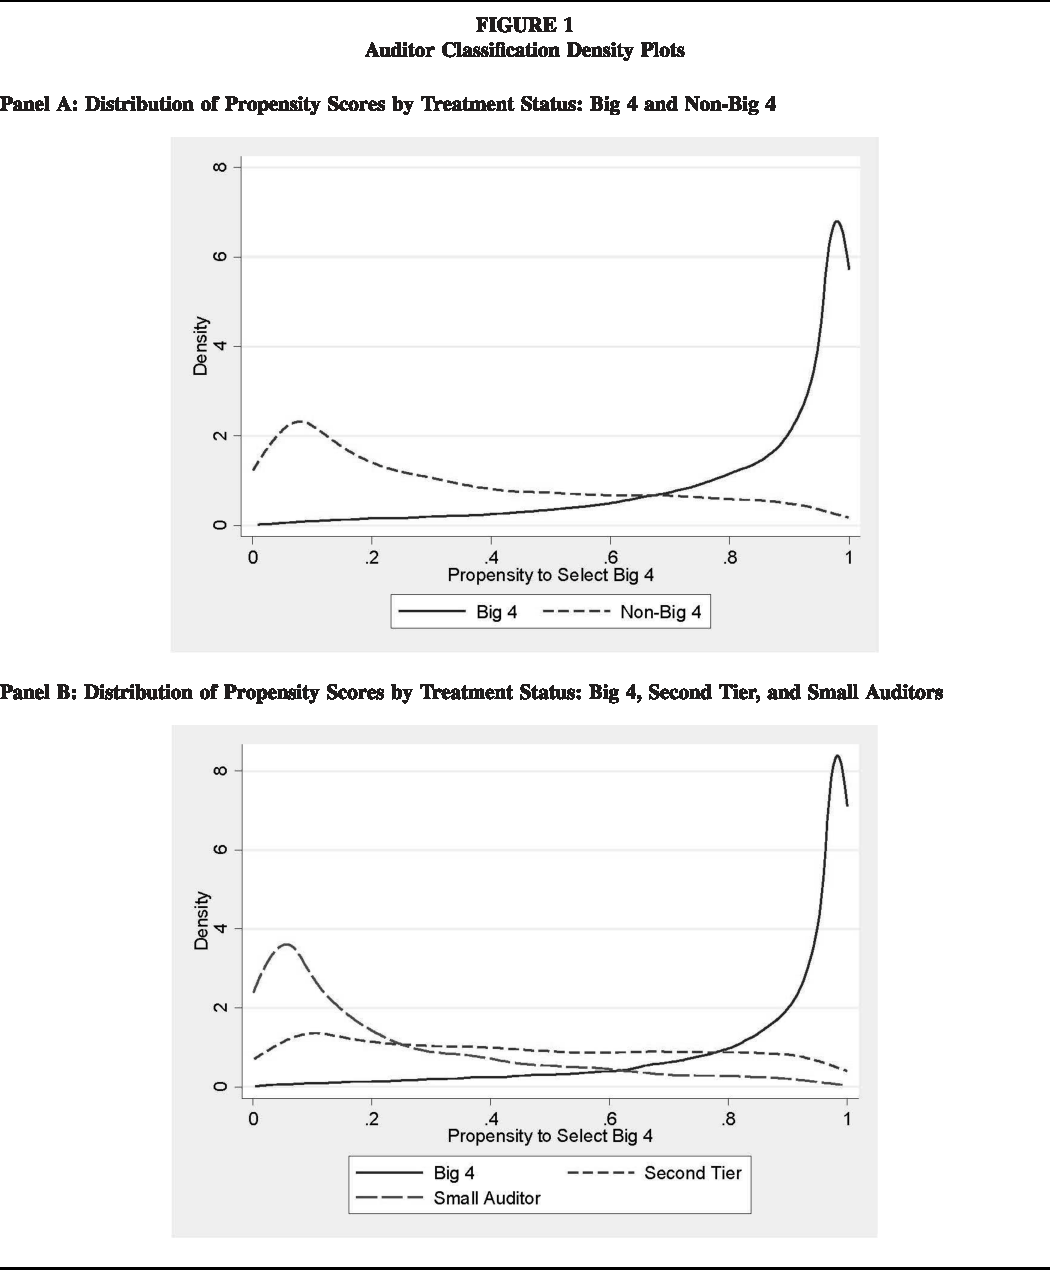
\includegraphics[width=16cm]{../fig/fig01.pdf}
\end{figure}

\begin{itemize}
 \item Big 4の監査法人のクライアントの傾向スコアは、0.9〜1の範囲内に集中し、非Big 4の監査法人のクライアントの傾向スコアは、0〜0.2に集中している。
 \item これは、共変量が割り当ての決定に大きく影響していることを示している。
 \item 結果的に、マッチングは、主として極端でない傾向スコアの範囲(ここでは、0.2〜0.9)の範囲内でなされることになる。
\end{itemize}

\paragraph{Second Tierを考慮して割り当てた場合の傾向スコアのプロット(Figure 1, Panel B)}

\begin{itemize}
 \item 非Big 4のクライアントから、Second Tierの監査法人のクライアントを識別する。
 \item この識別をしたプロットを見ると、Second Tierのクライアントは、0〜0.2の範囲内で、小規模監査法人のクライアントよりも傾向スコアが小さいが、0.2以上では小規模監査法人よりも大きな傾向スコアであることがわかる。
 \item これは、Second TierのクライアントがBig 4のクライアントとより多くマッチングが成立することを示す。
\end{itemize}

\paragraph{内部統制の弱さで割り当てた場合の傾向スコアの密度のプロット(Figure 2, Panel A)}

\begin{figure}
 \centering
 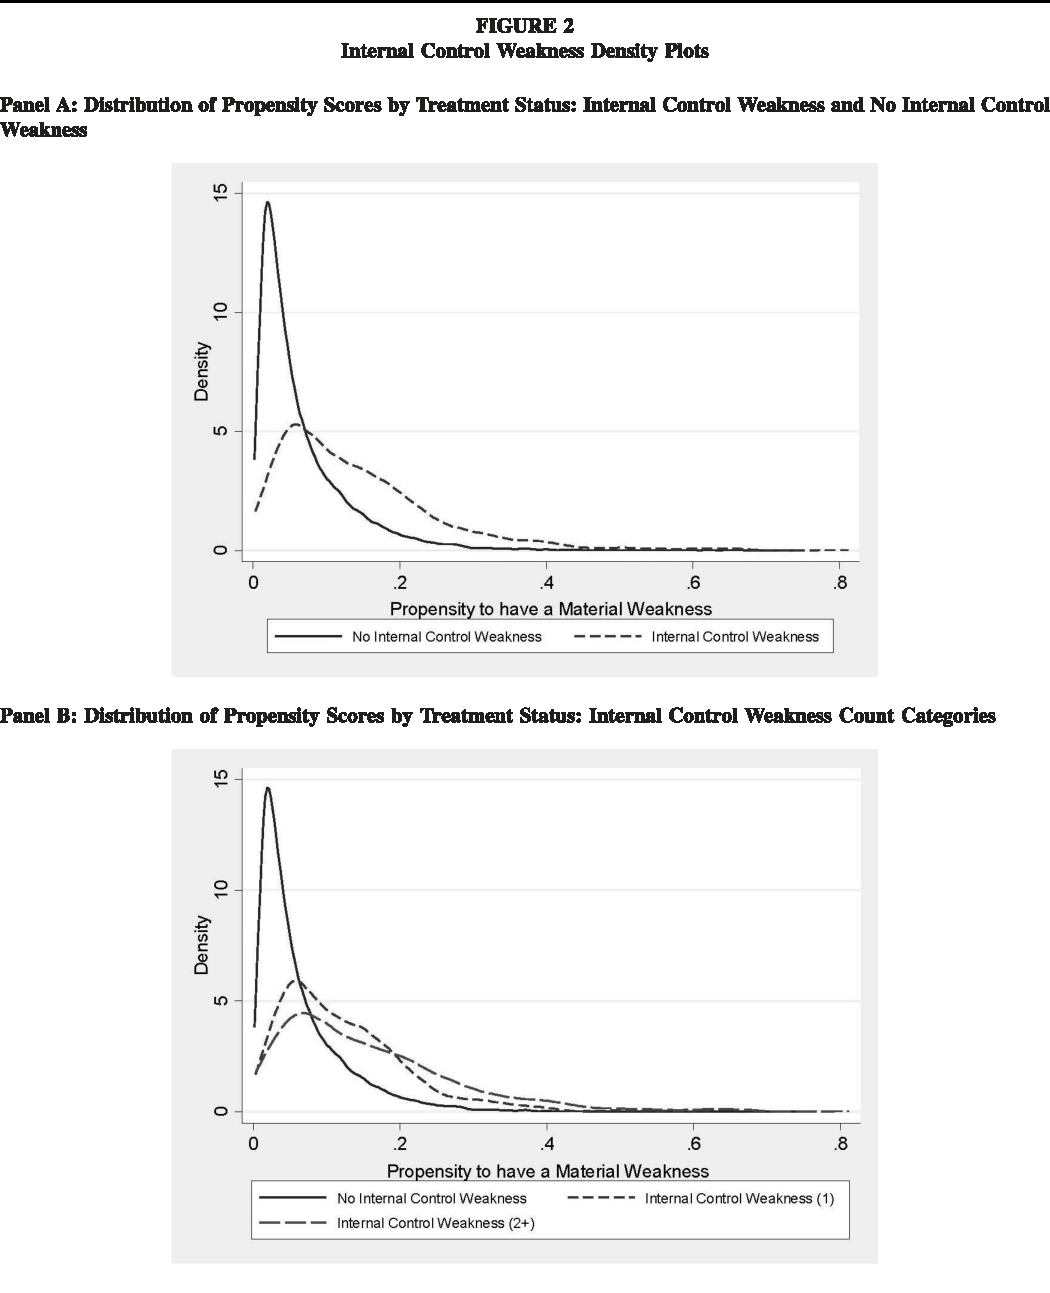
\includegraphics[width=16cm]{../fig/fig02.pdf}
\end{figure}

\begin{itemize}
 \item 監査法人の規模のときよりも、overlapの範囲が大きいことがわかる。
 \item Table 4のpseudo-${\rm R^2}$も、低い値であることもこのことを示唆している。
\end{itemize}

\paragraph{内部統制の弱さの判定を詳細にした場合の傾向スコアの密度のプロット(Figure 2, Panel B)}

\begin{itemize}
 \item 内部統制の弱さの判定をより詳細にする(No ICW、1 ICW、2+ICW)。
 \item 監査法人の規模の場合と同様に、overlapは、No ICWと2+ICWの間よりも、No ICWと1 ICWの間の方がより大きいことがわかる。
\end{itemize}

\paragraph{アナリストのフォローで割り当てた場合の傾向スコアの密度のプロット(Figure 3, Panel A)}

\begin{itemize}
 \item 監査法人の場合と同様に、処置群と対照群との間で傾向スコアの密度の範囲は異なっており、overlapが限定的なものであることがわかる。
\end{itemize}

\paragraph{アナリストのフォロー数を詳細にした場合の傾向スコアの密度のプロット(Figure 3, Panel B)}

\begin{itemize}
 \item アナリストのフォロー数を詳細にみる(1〜5人、6〜10人、11人以上)。
 \item プロットした結果、アナリストの数が少なければ少ないほど、アナリストに全くフォローされてない観測値とのoverlapが大きくなることがわかる。
 \item これは、マッチングがフォローしているアナリストの数の少ない企業となされる可能性が高いことを示している。
\end{itemize}

\subsection*{Matching without Replacement}

置き換えを認めず、1対1でマッチングを行う。

\paragraph{サンプルの構成(Table 5, Panel A)}

\begin{itemize}
 \item 置き換えをせず1対1でマッチングすると、かなりの数の観測値を除去することになる。
 \item 事実、“full sample”を比較して、監査法人の規模で30\%、内部統制の弱さで14\%、アナリストのフォローで28\%のサンプルしか確保できなかった。
 \item また、マッチングしたサンプルは、Second Tierのクライアントや、アナリストのフォロー数が少ない観測値で構成されていることもわかる。
  \begin{itemize}
   \item サンプルが小さいことは、外的な妥当性を減少させる、もしくは欠落させてしまう可能性を有している。
  \end{itemize}
\end{itemize}

\paragraph{MRとPSM間における共変量とATEの比較(Table 5, Panel B)}

\begin{itemize}
 \item 共変量は、PSMを行うことにより、バランスが向上していることがわかる。
  \begin{itemize}
   \item これは、MRにおいて、処置群と対照群の相違が残ったまま、ATEを推定していることを示す。
  \end{itemize}
 \item 裁量的会計発生高を従属変数とした場合、MRのATEはすべて有意であるが、PSMはすべて非有意であり、Chow(1960)の検定も、すべての係数間で有意である。
 \item 一方、財務諸表の再報告を従属変数とした場合は、MRとPSMのATEともにすべて類似した結果を示すが、係数を比較すると、有意な差が検出されるものが存在している。
\end{itemize}

\paragraph{まとめ}
\begin{itemize}
 \item 以上の分析から、MRとPSMでは推定される ATEが有意に異なっていることが明らかとなった。
 \item もし、PSMのみで分析すると、監査法人の規模、内部統制の弱さ、およびアナリストのフォローは、財務報告の質に影響を与えていないという結果のみを得ることになる。
 \item しかし、この ``帰無仮説を採択する'' (accept the null hypothesis) のは結論を急ぎ過ぎ (premature) であるかもしれない。
 \item 以下で、PSMの手法を変更することで、結果が変化することを示す。
\end{itemize}

\subsection*{Matching with Replacement}

置き換えを認めて、1対1でマッチングを行う。

\paragraph{サンプルの構成(Table 6, Panel B)}

\begin{itemize}
 \item (2)列目は、サンプルサイズが小さい方の群を処置群とし、サンプルサイズの大きな方の群にマッチングの置き換えを認める場合の結果である(Panel A)。
 \item サンプルサイズが大きくなっており、キャリパー距離(0.03)の間でより多くの対照群の観測値がマッチングしていることがわかる。
 \item (3)列目は、サンプルサイズの大きな方の群を処置群とし、サンプルサイズの小さい方の群にマッチングの置き換えを認める場合の結果である。
 \item サンプルサイズがかなり大きくなっており、ウェイトがいずれも5以上であることから、対照群の観測値がより多くの回数マッチングしていることがわかる。
 \item マッチングの手法ごとにサンプルの構成を比較した結果、9個の比較中8個で有意な差が認められる。
 \item 特に、Second Tierのクライアントの割合と、アナリストのフォロー数の平均値は、マッチングの手法間で顕著な差がある。
  \begin{itemize}
   \item マッチング手法の違いが、サンプルサイズとサンプルの構成に影響を与えてしまうことが示唆されている。
  \end{itemize}
\end{itemize}

\paragraph{ATEの比較(Table 6, Panel B, C)}

\begin{itemize}
 \item 監査法人の規模で割り当てた場合の結果は、いずれも非有意である。
 \item しかし、ATEの差が有意に検出されているものが存在する(6個の比較中3個)。
 \item 内部統制の弱さ、およびアナリストのフォローで割り当てた場合の結果は、マッチングの手法ごとに異なっており、ATEの差も有意に検出されているものがある(12個の比較中7個)。
  \begin{itemize}
   \item マッチングの手法が統計的な結果に影響を与えてしまう。
  \end{itemize}
\end{itemize}

\subsection*{The Influence of Matching Variables on Estimates of the ATE}

\paragraph{変数を置き換えてマッチングを行なった場合のサンプルの構成(Table 7, Panel A)}

\begin{itemize}
 \item 企業規模を示す変数を、総資産の自然対数($\mathit{LNASSETS}_{it}$)から時価総額の自然対数($\mathit{LNMARKET}_{it}$)に入れ替える。
 \item マッチングの手法間でサンプルを比較すると、共通の観測値は、58.9〜71.4\%の割合である。
 \item さらに、内部統制の弱さで割り当てた場合の対照群(内部統制の弱さが指摘されていない観測値)は、マッチングの手法間で、わずか18.2\%しかサンプルが共通してない。
\end{itemize}

\paragraph{変数を置き換えてマッチングを行なった場合のATE(Table 7, Panel B)}

\begin{itemize}
 \item $\mathit{LNASSETS}_{it}$のATEよりも、$\mathit{LNMARKET}_{it}$のATEの方が、有意であるものが多いことがわかる。
 \item 特に、アナリストのフォローで割り当てとし、財務諸表の再報告を従属変数とした時のATEは、Table 5の全サンプルとマッチングサンプルで非有意だったにもかかわらず、変数を置き換えると有意な結果が確認される。
 \item Chow(1960)の検定によれば、6個の比較中、3個でATEが有意な差であることが確認される。
\end{itemize}

\paragraph{変数を追加してマッチングを行った場合の結果(Table 8)}

\begin{itemize}
 \item 以下のとおり、変数を追加してマッチングを行う。
  \begin{itemize}
   \item 監査法人の規模:営業活動にかかるキャッシュフロー($\mathit{CFO}_{it}$)、海外売上高($\mathit{FOREIGN}_{it}$)
   \item 内部統制の弱さ:損失ダミー($\mathit{LOSS}_{it}$)
   \item アナリストのフォロー:$\mathit{LNMARKET}_{it}$
  \end{itemize}
 \item このマッチングからATEを求めた結果は、(2)列目と(5)列目に示されているが、いずれも有意であることがわかる。
 \item さらに以下のとおり変数を追加する。
  \begin{itemize}
   \item 監査法人の規模:$\mathit{LNASSETS}_{it-1}$、$LOSS_{it}$、棚卸資産($\mathit{INVENTORY}_{it}$)
   \item 内部統制の弱さ:$\mathit{FOREIGN}_{it}$
   \item アナリストのフォロー:$\mathit{BTM}_{it-1}$
  \end{itemize}
 \item 以上でマッチングし、ATEを求めた結果は、(3)列目と(6)列目に示されているが、これまでの検証で一貫して有意である内部統制の弱さで割り当て、財務諸表の再報告を従属変数としたATE以外、すべて非有意である。
  \begin{itemize}
   \item 以上から、ATEの推定は、PSMのモデルの設定から影響を受けやすいことが明らかである。
  \end{itemize}
 \item 以上の変数の選択は、結果の頑健性を示すために、``事後的''に選択されたことに留意するべきである。
 \item すべての$X$は、結果に同じような影響を与えるとは限らない。
  \begin{itemize}
   \item ここから、PSMの変数の選択において、十分な考慮をするこの重要さが示唆される。
  \end{itemize}
\end{itemize}
